\documentclass[11pt,letterpaper]{article}

% ---------------------------------------------------------------
% Paquetes
% ---------------------------------------------------------------
\usepackage[spanish,es-tabla]{babel}
\usepackage[utf8]{inputenc}
\usepackage[margin=2.5cm]{geometry}
\usepackage{graphicx}
\usepackage{booktabs}
\usepackage{multirow}
\usepackage{longtable}
\usepackage{array}
\usepackage{xcolor}
\usepackage{titlesec}
\usepackage{enumitem}
\usepackage{amsmath}
\usepackage{caption}
\usepackage{fancyhdr}
\usepackage{parskip}
\usepackage[hidelinks,colorlinks=true,linkcolor=black,citecolor=black,urlcolor=blue!50!black]{hyperref}

\definecolor{sscobalt}{HTML}{1B6CA8}
\definecolor{sscoral}{HTML}{E2711D}
\definecolor{ssgray}{HTML}{4A4A4A}

\titleformat{\section}{\normalfont\Large\bfseries\color{sscobalt}}{\thesection.}{0.6em}{}
\titleformat{\subsection}{\normalfont\large\bfseries\color{ssgray}}{\thesubsection.}{0.6em}{}
\titleformat{\subsubsection}{\normalfont\normalsize\bfseries\itshape}{\thesubsubsection.}{0.5em}{}

\pagestyle{fancy}
\fancyhf{}
\fancyhead[L]{\small SteamSense Pro --- Informe técnico y estrategia de fidelización}
\fancyhead[R]{\small\thepage}
\renewcommand{\headrulewidth}{0.4pt}

\setlength{\parindent}{0pt}
\setlength{\parskip}{0.5em}

\newcommand{\code}[1]{\texttt{\small #1}}

\title{
  \vspace{-1.5cm}
  {\color{sscobalt}\rule{\linewidth}{2pt}}\\[0.4cm]
  {\Huge\bfseries SteamSense Pro}\\[0.2cm]
  {\Large Predicción de abandono y segmentación de jugadores de RPG \\ para estrategias de fidelización en Steam}\\[0.3cm]
  {\color{sscobalt}\rule{\linewidth}{1pt}}
}
\author{Juan Miguel Galán Olivares}
\date{Agosto de 2026}

\begin{document}

\maketitle
\thispagestyle{empty}

\begin{abstract}
\noindent
Millones de personas compran videojuegos de rol (RPG) en Steam cada año, pero una fracción considerable los abandona antes de terminarlos o incluso sin haberlos jugado. Este fenómeno representa una pérdida de valor tanto para los jugadores, que gastan dinero en productos que no disfrutan, como para los estudios y publishers, que ven caer la retención y el gasto recurrente de su base de usuarios. \textbf{SteamSense Pro} es un sistema de análisis de datos y aprendizaje automático que, a partir del historial público de un jugador en Steam, (1) recomienda qué RPGs tienen menor probabilidad de ser abandonados antes de comprarlos, (2) advierte sobre el riesgo de abandono de los juegos que la persona ya posee, y (3) identifica su perfil de consumo mediante \textit{clustering} no supervisado. El proyecto integra datos de la API de Steam, SteamSpy y HowLongToBeat sobre más de 15{,}700 títulos y cerca de 30 millones de registros jugador--juego, para entrenar dos modelos de clasificación (LightGBM, ganador con \textit{Average Precision} de 0.966 y 0.999 respectivamente) y un modelo de mezcla de gaussianas (GMM) que segmenta a los jugadores en tres perfiles: \emph{Dedicado}, \emph{Coleccionista Dormido} y \emph{Coleccionista Masivo}. El resultado se despliega como una aplicación interactiva en Streamlit con un asistente conversacional, y da lugar a una estrategia de fidelización accionable tanto para jugadores individuales como para estudios y publishers de videojuegos.
\end{abstract}

\tableofcontents

% ===================================================================
\section{Introducción}
% ===================================================================

Steam es la plataforma de distribución digital de videojuegos más grande del mundo, con un catálogo que incluye decenas de miles de títulos del género de rol (RPG, por \textit{role-playing game}). Este género se caracteriza por ofrecer experiencias largas, con una historia principal, contenido secundario y, en muchos casos, cientos de horas de contenido adicional. Esa misma extensión es también su mayor riesgo comercial: comprar un RPG es una decisión de alto compromiso de tiempo, y una parte importante de los jugadores termina abandonando el juego antes de completar ni siquiera la historia principal, o sin llegar a iniciarlo.

Para los jugadores, esto se traduce en dinero y tiempo mal invertidos y en una experiencia de descubrimiento de catálogo poco eficiente entre miles de opciones similares. Para los estudios de desarrollo y los publishers, el abandono temprano reduce la retención, el boca a boca positivo, las probabilidades de recompra de secuelas o contenido descargable (DLC), y en última instancia el valor de vida del cliente (\textit{customer lifetime value}). SteamSense Pro nace para atender ambos lados del problema con una misma base analítica: usar el historial de juego públicamente disponible en Steam para predecir, antes y después de la compra, la probabilidad de que un jugador abandone un RPG, y para caracterizar su estilo de consumo de forma que la recomendación y la comunicación con él puedan ajustarse a su perfil real.

El proyecto combina tres componentes de aprendizaje automático ---dos modelos de clasificación supervisada y un modelo de \textit{clustering} no supervisado (GMM)--- entrenados sobre datos reales extraídos de la API de Steam, SteamSpy y HowLongToBeat, y los integra en una aplicación web (Streamlit) con un asistente conversacional que traduce las predicciones en recomendaciones concretas para el usuario final.

% ===================================================================
\section{Planteamiento del problema}
% ===================================================================

El problema central que aborda SteamSense Pro puede formularse en dos preguntas conectadas:

\begin{enumerate}[label=(\roman*)]
  \item \textbf{Antes de la compra:} dado el historial de juego de una persona en Steam (qué juegos posee, cuánto los ha jugado, cuán activa ha sido recientemente), ¿qué RPGs de un catálogo de miles de títulos tienen la menor probabilidad de ser abandonados por esa persona en particular?
  \item \textbf{Después de la compra:} para los RPGs que la persona ya posee, ¿cuáles corren mayor riesgo de quedar inconclusos, de forma que se puedan priorizar acciones de reenganche (recordatorios, recomendaciones de contenido, comunicación dirigida) antes de perder al jugador por completo?
\end{enumerate}

\subsection{Definición operativa de ``abandono''}

Un jugador se considera en situación de \textbf{abandono} respecto de un RPG cuando cumple simultáneamente dos condiciones observables en los datos de Steam:

\begin{itemize}
  \item No ha jugado el título en las últimas dos semanas (\code{horas\_2\_semanas == 0}).
  \item Las horas totales jugadas están por debajo de un umbral de finalización razonable del juego (\code{horas\_totales < umbral\_completado}), donde dicho umbral se define, en orden de preferencia, como las horas de finalización al 100\% (\code{completionist}), o si ese dato no está disponible, las horas de historia principal más contenido secundario (\code{main\_extra}), o en su defecto solo la historia principal (\code{main\_story}), según los datos de HowLongToBeat.
\end{itemize}

Esta definición se aplica de forma ligeramente distinta según el momento de la decisión de negocio: el \textbf{Modelo 1 (precompra)} exige además haber jugado al menos una hora (para no confundir ``nunca lo probé'' con ``lo empecé y lo dejé''), mientras que el \textbf{Modelo 2 (postcompra)} incluye también los casos de compra sin ningún uso, porque desde la perspectiva de un juego ya adquirido, \emph{no jugarlo en absoluto} es en sí mismo la señal de riesgo más temprana y más accionable.

La relevancia del problema es doble: desde la perspectiva del \textbf{jugador}, se trata de un problema de descubrimiento y de gasto informado en un catálogo con miles de RPGs de duración y calidad muy dispares; desde la perspectiva de la \textbf{industria}, se trata de un problema de retención de clientes en un mercado donde adquirir un nuevo jugador es sustancialmente más costoso que conservar uno existente, y donde el abandono temprano es una señal de alerta que hoy no se explota de forma sistemática por falta de modelos predictivos accesibles a estudios pequeños y medianos.

% ===================================================================
\section{Estrategia (resumen)}
% ===================================================================

La estrategia completa ---accionables, usuarios objetivo y usabilidad del modelo--- se desarrolla en detalle en la Sección~\ref{sec:estrategia}. En síntesis, SteamSense Pro traduce las predicciones de los tres modelos en una estrategia de \textbf{fidelización de jugadores de RPG} con valor para dos tipos de usuario: los \textbf{jugadores}, a quienes ayuda a elegir mejor y a no abandonar lo que ya compraron, y las \textbf{empresas del sector} (estudios, publishers y la propia plataforma), a quienes ofrece una capa de inteligencia de retención que hoy requeriría equipos de datos propios.

% ===================================================================
\section{Descripción de los datos}
% ===================================================================

Los datos del proyecto provienen de tres fuentes públicas, combinadas mediante un proceso de recolección progresiva con puntos de control (\textit{checkpoints}) para tolerar cortes de conexión y límites de tasa de las APIs:

\begin{itemize}
  \item \textbf{SteamSpy} (SteamSpy, s.f.) (\url{https://steamspy.com/api.php}): catálogo de juegos del género RPG (\code{appid}, nombre, desarrollador, publisher, rango estimado de propietarios (\emph{owners}), horas promedio/mediana jugadas, precio, etiquetas e idiomas). Es la fuente que define el universo de \textbf{15{,}784 títulos RPG} sobre el que trabaja el proyecto.
  \item \textbf{HowLongToBeat} (HowLongToBeat, s.f.) (vía el paquete \code{howlongtobeatpy}): duración de cada título en tres niveles ---\code{main\_story} (solo historia principal), \code{main\_extra} (historia más contenido secundario razonable) y \code{completionist} (100\% de finalización)---. Tras el cruce por nombre estandarizado con el catálogo de SteamSpy y exigir \code{main\_story > 0}, quedan \textbf{3{,}475 juegos} con duración confiable, que son la base de los modelos de precompra.
  \item \textbf{Steam Web API} (Valve Corporation, s.f.): como Steam no ofrece un endpoint que devuelva directamente ``qué jugadores tienen este juego'', el proyecto usa las reseñas públicas (\code{/appreviews/\{appid\}}) como semilla para descubrir \code{steamid} reales, y luego expande ese conjunto mediante las listas de amigos (\code{GetFriendList}) de esos mismos jugadores. Para cada \code{steamid} resultante se obtiene su biblioteca completa (\code{GetOwnedGames}: juegos poseídos, horas totales y horas en las últimas dos semanas) y su perfil público (\code{GetPlayerSummaries}).
\end{itemize}

\subsection{Volumen y calidad de los datos}

Tras deduplicar y limpiar los registros jugador--juego, el conjunto de trabajo alcanza aproximadamente \textbf{29.97 millones de filas} jugador--juego (biblioteca completa, no solo RPG) correspondientes a \textbf{70{,}734 jugadores únicos}. Al filtrar solo los títulos del catálogo RPG con duración confiable, el conjunto se reduce a \textbf{3{,}906{,}468 registros} jugador--RPG sobre \textbf{3{,}122 títulos únicos}.

La calidad de los datos presenta dos limitaciones relevantes, tratadas explícitamente en el procesamiento (Sección~\ref{sec:procesamiento}):

\begin{itemize}
  \item Solo el 49\% del catálogo SteamSpy (7{,}751 de 15{,}784 juegos) tiene datos de duración en HowLongToBeat, y de esos, solo 3{,}475 superan los filtros de calidad de nombre y de horas de historia $>0$. El resto del catálogo no puede usarse para los modelos de precompra por falta de un umbral de finalización confiable.
  \item Los rangos de propietarios de SteamSpy son estimaciones por buckets (por ejemplo, ``50{,}000{,}000 .. 100{,}000{,}000''), no cifras exactas, por lo que se tratan como una variable ordinal aproximada (ver \code{log\_owners} en la Sección~\ref{sec:procesamiento}) y no como un conteo preciso de ventas.
\end{itemize}

Estos datos son suficientemente relevantes para el problema porque combinan exactamente las dos dimensiones que definen el abandono: \emph{cuánto necesita jugarse un título para considerarse terminado} (HowLongToBeat) y \emph{cuánto ha jugado realmente cada persona y qué tan reciente fue esa actividad} (Steam Web API), enriquecidos con el contexto de toda su biblioteca (SteamSpy + Steam Web API) para caracterizar su comportamiento general como jugador, no solo su relación con un título aislado.

% ===================================================================
\section{Análisis exploratorio de datos}
% ===================================================================

El análisis exploratorio se realizó en dos niveles: a nivel de \textbf{catálogo de juegos} y a nivel de \textbf{comportamiento de jugadores}.

\subsection{Catálogo de juegos}

Sobre los 4{,}185 juegos del catálogo con horas de historia principal registradas en HowLongToBeat (un superconjunto de los 3{,}475 que además superan el filtro de emparejamiento exacto de nombres usado para modelar), la distribución de horas de historia principal es marcadamente asimétrica a la derecha (Figura~\ref{fig:main_story}): la mayoría de los RPGs se completan en menos de 20 horas de historia principal, con una cola larga de títulos que superan las 60--90 horas. Este patrón motivó el uso de percentiles (en lugar de la media) para evaluar valores extremos, y de una transformación logarítmica para la variable de propietarios estimados, cuya distribución de conteos abarca varios órdenes de magnitud.

\begin{figure}[h!]
  \centering
  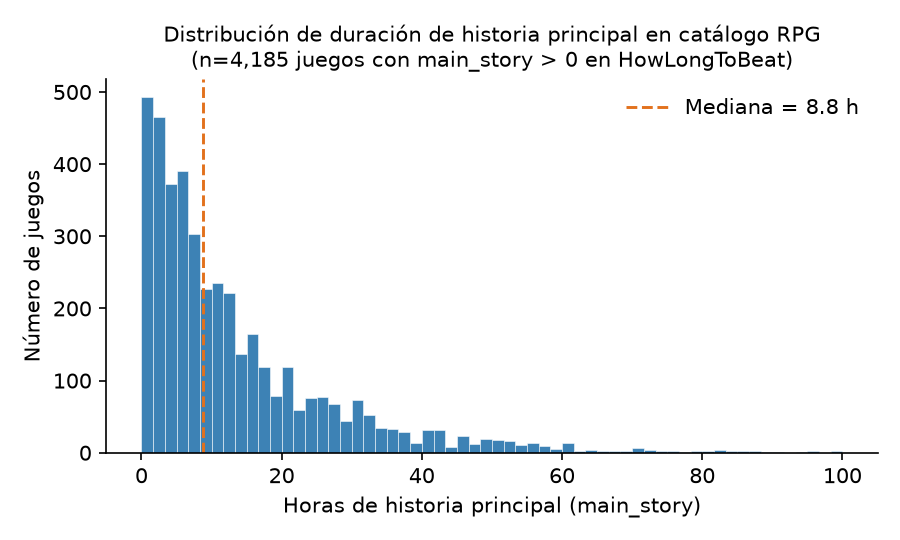
\includegraphics[width=0.75\linewidth]{fig_main_story_dist.png}
  \caption{Distribución de horas de historia principal en el catálogo RPG con datos confiables de HowLongToBeat.}
  \label{fig:main_story}
\end{figure}

Un hallazgo relevante del EDA es que, al comparar las tres métricas de duración de HowLongToBeat, el \textbf{36.6\% de los juegos} (1{,}272 de 3{,}475) presenta inconsistencias respecto de la jerarquía esperada \(\text{main\_story} \le \text{main\_extra} \le \text{completionist}\) ---por ejemplo, un \code{main\_story} reportado como mayor que el \code{main\_extra}---, producto de cómo la comunidad de HowLongToBeat reporta tiempos de forma independiente para cada categoría. Este hallazgo fue el detonante directo de las reglas de corrección aplicadas en la etapa de procesamiento (Sección~\ref{sec:procesamiento}).

También se generaron histogramas y estimaciones de densidad (KDE) sobre las variables de duración y de propietarios para identificar posibles distribuciones bimodales o multimodales, con el objetivo de anticipar qué variables serían buenas candidatas para separar segmentos de jugadores en la etapa de \textit{clustering}, además de un resumen estadístico descriptivo completo (media, mediana, dispersión, valores nulos) tanto del catálogo de juegos como del comportamiento de los jugadores.

\subsection{Comportamiento de los jugadores}

A nivel de jugador, el conjunto crudo de 31{,}295{,}960 registros jugador--juego se redujo a 29{,}972{,}160 tras eliminar duplicados y \code{appid} nulos. Las estadísticas descriptivas muestran una distribución de horas jugadas extremadamente concentrada en pocos títulos por jugador: la media de horas totales por juego es de 20.24 horas, pero con una desviación estándar de 483.3 horas, reflejo de que la mayoría de los juegos en una biblioteca típica de Steam se juegan poco o nada, mientras un número reducido de títulos concentra cientos o miles de horas. Del total de la biblioteca completa (no solo RPG), únicamente 223{,}505 registros muestran actividad en las últimas dos semanas, lo que confirma que el abandono ---en el sentido de inactividad reciente--- es la norma y no la excepción en el comportamiento típico de un jugador de Steam, y justifica por qué el problema de negocio (predecir abandono) es relevante a esta escala.

% ===================================================================
\section{Procesamiento de datos}
\label{sec:procesamiento}
% ===================================================================

El procesamiento de datos se dividió en limpieza del catálogo de juegos, corrección de inconsistencias de duración, e ingeniería de variables a nivel de jugador.

\subsection{Limpieza y estandarización}

\begin{itemize}
  \item \textbf{Emparejamiento de nombres:} los nombres de los juegos en SteamSpy y en HowLongToBeat no siempre coinciden textualmente (mayúsculas, acentos, comillas, subtítulos). Se aplicó una función de estandarización de texto y se conservaron solo los emparejamientos exactos tras la normalización, lo que redujo el catálogo utilizable de 15{,}784 a 3{,}475 juegos.
  \item \textbf{Corrección de la jerarquía de duración:} para los juegos con inconsistencias detectadas en el EDA (36.6\% del catálogo), se aplicaron dos reglas de corrección: (1) \(\text{main\_extra} \leftarrow \max(\text{main\_story}, \text{main\_extra})\), y (2) el valor de \code{completionist} se descarta (se marca como no disponible) cuando es cero o menor que \code{main\_extra}, por considerarse poco confiable. El umbral de finalización usado como referencia para definir abandono (\code{umbral\_completado}) se construye entonces en cascada: se usa \code{completionist} si es válido, si no \code{main\_extra}, y si tampoco está disponible, \code{main\_story}.
  \item \textbf{Transformación de propietarios estimados:} el rango de \code{owners\_estimado} de SteamSpy (texto tipo bucket) se convierte a un valor numérico de punto medio mediante un diccionario de 12 rangos fijos (de 10{,}000 a 75{,}000{,}000), y luego se aplica \(\text{log\_owners} = \log(1 + \text{owners\_punto\_medio})\) para reducir la asimetría extrema de esta variable antes de usarla como \textit{feature}.
\end{itemize}

\subsection{Ingeniería de variables}

A partir de los datos limpios se construyeron variables derivadas tanto a nivel de juego como a nivel de jugador:

\begin{itemize}
  \item \(\text{ratio\_extra\_vs\_historia} = \text{main\_extra} / \text{main\_story}\): mide qué tan grande es el contenido secundario de un título respecto a su historia principal, como \textit{proxy} de la ``densidad'' de contenido opcional.
  \item \(\text{pct\_completado\_historia} = \text{horas\_totales} / \text{main\_story}\): avance relativo de un jugador en un título específico.
  \item Variables agregadas por jugador (calculadas sobre \emph{toda} su biblioteca de Steam, no solo sus RPG, para capturar hábitos generales de consumo): número total de juegos poseídos (\code{num\_juegos\_totales}), horas totales acumuladas en toda la biblioteca (\code{horas\_totales\_todos\_juegos}), número de juegos con actividad en las últimas dos semanas (\code{num\_juegos\_activos}, también referida como \code{dispersion\_de\_atencion}), proporción de la biblioteca que está activa (\code{pct\_juegos\_activos}), número de RPGs poseídos del catálogo (\code{num\_rpg\_jugados}) y el promedio de avance relativo de historia en sus RPGs (\code{promedio\_pct\_completado\_historia\_global}).
  \item \textbf{Ajuste \textit{leave-one-out}:} dado que el conjunto de entrenamiento del Modelo 2 tiene una fila por cada par (jugador, RPG poseído), cada variable agregada de jugador se recalculó restando la contribución del propio juego de esa fila, para evitar que el modelo ``se vea a sí mismo'' dentro de su propio promedio (fuga de información). Esta corrección se aplicó a todas las variables agregadas salvo a \code{promedio\_pct\_completado\_historia\_global}, que por decisión explícita de diseño no se ajusta por \textit{leave-one-out}; se documenta como una limitación conocida del modelo (ver Sección~\ref{sec:conclusiones}).
  \item Para el Modelo 2 se añadieron además dos variables de corte temporal que evitan fuga de información desde el futuro: \(\text{horas\_hasta\_corte} = \text{horas\_totales} - \text{horas\_2\_semanas}\) y \(\text{pct\_avance\_hasta\_corte} = \text{horas\_hasta\_corte} / \text{main\_story}\), que representan el avance del jugador \emph{antes} de la ventana de las últimas dos semanas usada para etiquetar el abandono.
\end{itemize}

Con estas transformaciones se definieron tres conjuntos finales de variables: 11 \textit{features} para el Modelo 1, 13 para el Modelo 2 (las 11 anteriores más las dos variables de corte temporal), y 6 variables para el modelo de \textit{clustering} (las variables agregadas de jugador, sin las específicas de un juego individual).

Todo el conjunto de datos se dividió en entrenamiento, validación y prueba en proporción \textbf{60/20/20}, estratificando por la variable objetivo para preservar el desbalance de clases en las tres particiones.

% ===================================================================
\section{Modelación supervisada y no supervisada}
\label{sec:modelacion}
% ===================================================================

\subsection{Modelos supervisados: predicción de abandono}

Se entrenaron dos modelos de clasificación binaria independientes, ambos bajo el mismo esquema de búsqueda de hiperparámetros:

\begin{itemize}
  \item \textbf{Modelo 1 (precompra):} predice la probabilidad de que un jugador abandone un RPG que \emph{todavía no posee}, usando únicamente variables de su comportamiento general (biblioteca) y de las características del juego candidato. Entrenado sobre 1{,}133{,}070 registros (60\%), con un desbalance de clases de 85\% abandono / 15\% no abandono.
  \item \textbf{Modelo 2 (postcompra):} predice la probabilidad de abandono de un RPG que el jugador \emph{ya posee}, incluyendo casos de compra sin ningún uso. Entrenado sobre 2{,}343{,}880 registros (60\%), con un desbalance de clases de 93\% abandono / 7\% no abandono.
\end{itemize}

Para ambos modelos se construyó un mismo \textit{pipeline} de \code{scikit-learn} (Pedregosa et al., 2011): escalado de variables numéricas $\rightarrow$ eliminación de varianza casi nula (\code{VarianceThreshold}) $\rightarrow$ selección de variables (\code{SelectKBest}, prueba F) $\rightarrow$ clasificador. La búsqueda de hiperparámetros se realizó con \code{GridSearchCV} (validación cruzada de 4 particiones), optimizando \textbf{Average Precision} ---métrica preferida sobre \textit{accuracy} o incluso ROC-AUC dado el fuerte desbalance de clases y la importancia relativa de identificar bien la clase minoritaria (``no abandono'', el caso de negocio más valioso de acertar)---.

Se compararon cinco familias de modelos para el Modelo 1 (LightGBM [Ke et al., 2017], XGBoost [Chen \& Guestrin, 2016], K-Vecinos Más Cercanos, Regresión Logística y Análisis Discriminante Lineal) y cuatro para el Modelo 2 (las mismas, sin Regresión Logística, descartada de antemano por su desempeño consistentemente inferior frente a los modelos de árboles en la búsqueda preliminar del Modelo 1). Los resultados completos de la búsqueda de hiperparámetros, con la mejor combinación de escalador e hiperparámetros por familia de modelo, se resumen en la Tabla~\ref{tab:grid1} (Modelo 1) y la Tabla~\ref{tab:grid2} (Modelo 2), y se comparan visualmente en la Figura~\ref{fig:gridsearch}.

\begin{table}[h!]
\centering
\small
\caption{Mejor \textit{Average Precision} (validación cruzada) por familia de modelo --- Modelo 1 (precompra).}
\label{tab:grid1}
\begin{tabular}{@{}llrl@{}}
\toprule
Familia de modelo & Mejor escalador & AP (CV) & Hiperparámetros clave \\
\midrule
\textbf{LightGBM} & RobustScaler & \textbf{0.9664} & lr=0.1, n\_est.=350, num\_leaves=31, k=11 \\
XGBoost & RobustScaler/Standard/MinMax & 0.9643 & lr=0.1, max\_depth=5, n\_est.=300, k=11 \\
KNN & RobustScaler & 0.9341 & n\_neighbors=9, weights=distance, k=11 \\
Regresión Logística & StandardScaler & 0.9115 & C=10, k=11 \\
LDA & (indiferente) & 0.8989 & shrinkage=auto, solver=lsqr, k=11 \\
\bottomrule
\end{tabular}
\end{table}

\begin{table}[h!]
\centering
\small
\caption{Mejor \textit{Average Precision} (validación cruzada) por familia de modelo --- Modelo 2 (postcompra).}
\label{tab:grid2}
\begin{tabular}{@{}llrl@{}}
\toprule
Familia de modelo & Mejor escalador & AP (CV) & Hiperparámetros clave \\
\midrule
\textbf{LightGBM} & RobustScaler & \textbf{0.9992} & lr=0.1, n\_est.=350, num\_leaves=31, k=11 \\
XGBoost & RobustScaler & 0.9991 & lr=0.1, max\_depth=5, n\_est.=300, k=11 \\
KNN & RobustScaler & 0.9938 & n\_neighbors=9, weights=distance, k=11 \\
LDA & (indiferente) & 0.9635 & shrinkage=auto, solver=lsqr, k=11 \\
\bottomrule
\end{tabular}
\end{table}

\begin{figure}[h!]
  \centering
  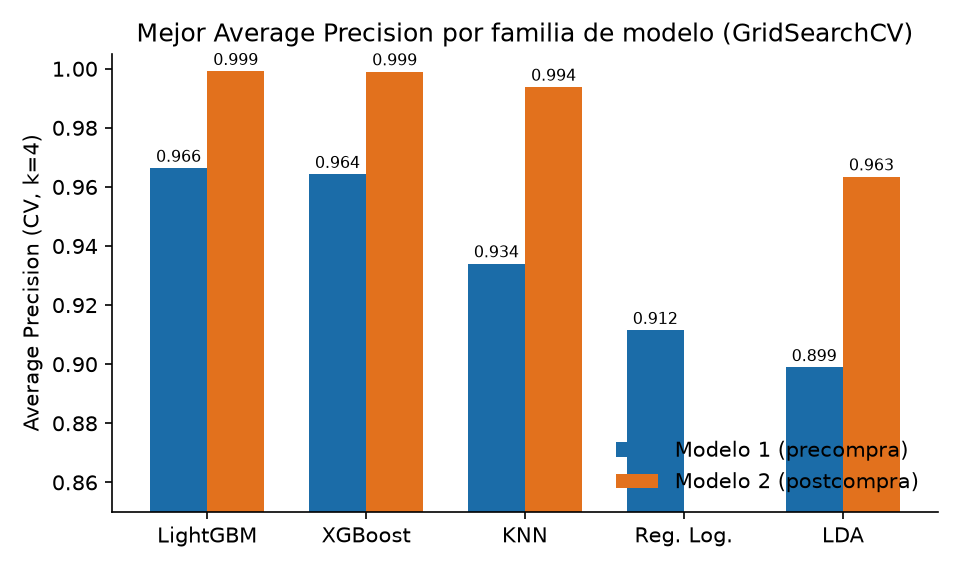
\includegraphics[width=0.85\linewidth]{fig_gridsearch_comparacion.png}
  \caption{Comparación del mejor \textit{Average Precision} obtenido por cada familia de modelo, para ambos problemas de clasificación.}
  \label{fig:gridsearch}
\end{figure}

\subsubsection{Selección y justificación del modelo final}

En ambos problemas, \textbf{LightGBM} resultó el modelo ganador. La elección no se basó solo en el \textit{Average Precision} de validación cruzada (Tablas~\ref{tab:grid1} y~\ref{tab:grid2}), sino en la evaluación de un conjunto completo de métricas (\textit{accuracy}, precisión, \textit{recall}, F1, ROC-AUC y Average Precision) sobre las tres particiones de entrenamiento, validación y prueba, para todas las familias de modelos evaluadas: la Tabla~\ref{tab:full_m1} muestra este detalle para el Modelo 1 y la Tabla~\ref{tab:full_m2} para el Modelo 2.

\begin{table}[h!]
\centering
\footnotesize
\caption{Métricas completas por partición y familia de modelo --- Modelo 1 (precompra).}
\label{tab:full_m1}
\begin{tabular}{@{}llrrrrrr@{}}
\toprule
Modelo & Partición & Exactitud & Precisión & Recall & F1 & ROC-AUC & AP \\
\midrule
\multirow{3}{*}{\textbf{LightGBM}}
  & Entrenamiento & 0.78 & 0.95 & 0.79 & 0.86 & 0.86 & 0.97 \\
  & Validación    & 0.78 & 0.95 & 0.79 & 0.86 & 0.85 & 0.97 \\
  & Prueba        & \textbf{0.78} & \textbf{0.95} & \textbf{0.79} & \textbf{0.86} & \textbf{0.85} & \textbf{0.97} \\
\addlinespace
\multirow{3}{*}{XGBoost}
  & Entrenamiento & 0.78 & 0.94 & 0.78 & 0.86 & 0.85 & 0.97 \\
  & Validación    & 0.77 & 0.94 & 0.78 & 0.86 & 0.85 & 0.96 \\
  & Prueba        & 0.78 & 0.94 & 0.78 & 0.86 & 0.84 & 0.96 \\
\addlinespace
\multirow{3}{*}{KNN}
  & Entrenamiento & 1.00 & 1.00 & 1.00 & 1.00 & 1.00 & 1.00 \\
  & Validación    & 0.86 & 0.88 & 0.97 & 0.92 & 0.77 & 0.94 \\
  & Prueba        & 0.86 & 0.88 & 0.97 & 0.92 & 0.77 & 0.94 \\
\addlinespace
\multirow{3}{*}{Regresión Logística}
  & Entrenamiento & 0.58 & 0.90 & 0.57 & 0.70 & 0.66 & 0.91 \\
  & Validación    & 0.58 & 0.90 & 0.57 & 0.70 & 0.66 & 0.91 \\
  & Prueba        & 0.58 & 0.90 & 0.57 & 0.70 & 0.66 & 0.91 \\
\addlinespace
\multirow{3}{*}{LDA}
  & Entrenamiento & 0.85 & 0.85 & 1.00 & 0.92 & 0.63 & 0.90 \\
  & Validación    & 0.85 & 0.85 & 1.00 & 0.92 & 0.62 & 0.90 \\
  & Prueba        & 0.85 & 0.85 & 1.00 & 0.92 & 0.62 & 0.90 \\
\bottomrule
\end{tabular}
\end{table}

\begin{table}[h!]
\centering
\footnotesize
\caption{Métricas completas por partición y familia de modelo --- Modelo 2 (postcompra).}
\label{tab:full_m2}
\begin{tabular}{@{}llrrrrrr@{}}
\toprule
Modelo & Partición & Exactitud & Precisión & Recall & F1 & ROC-AUC & AP \\
\midrule
\multirow{3}{*}{\textbf{LightGBM}}
  & Entrenamiento & 0.97 & 1.00 & 0.97 & 0.98 & 0.99 & 1.00 \\
  & Validación    & 0.97 & 1.00 & 0.97 & 0.98 & 0.99 & 1.00 \\
  & Prueba        & \textbf{0.97} & \textbf{1.00} & \textbf{0.97} & \textbf{0.98} & \textbf{0.99} & \textbf{1.00} \\
\addlinespace
\multirow{3}{*}{XGBoost}
  & Entrenamiento & 0.96 & 1.00 & 0.96 & 0.98 & 0.99 & 1.00 \\
  & Validación    & 0.96 & 1.00 & 0.96 & 0.98 & 0.99 & 1.00 \\
  & Prueba        & 0.96 & 1.00 & 0.96 & 0.98 & 0.99 & 1.00 \\
\addlinespace
\multirow{3}{*}{KNN}
  & Entrenamiento & 1.00 & 1.00 & 1.00 & 1.00 & 1.00 & 1.00 \\
  & Validación    & 0.97 & 0.98 & 0.99 & 0.98 & 0.96 & 0.99 \\
  & Prueba        & 0.97 & 0.98 & 0.99 & 0.98 & 0.96 & 0.99 \\
\addlinespace
\multirow{3}{*}{LDA}
  & Entrenamiento & 0.93 & 0.93 & 1.00 & 0.96 & 0.71 & 0.96 \\
  & Validación    & 0.93 & 0.93 & 1.00 & 0.96 & 0.71 & 0.96 \\
  & Prueba        & 0.93 & 0.93 & 1.00 & 0.96 & 0.71 & 0.96 \\
\bottomrule
\end{tabular}
\end{table}

Un patrón que merece una lectura cuidadosa en ambas tablas es el de \textbf{K-Vecinos Más Cercanos (KNN)}: sus métricas de entrenamiento son perfectas o casi perfectas (1.00 en las seis métricas), muy por encima de sus propios valores de validación y prueba. Esto no es una señal genuina de capacidad predictiva superior, sino un artefacto conocido de evaluar un modelo basado en distancias sobre su propio conjunto de entrenamiento: el vecino más cercano de un punto de entrenamiento suele ser él mismo (distancia cero), lo que infla artificialmente sus métricas de entrenamiento. El desempeño real de KNN es el que se observa en validación y prueba, donde cae varios puntos por debajo de LightGBM y XGBoost en ambos modelos.

Para el modelo ganador (LightGBM), el reporte de clasificación detallado por clase y partición se muestra en la Tabla~\ref{tab:cr_m1} (Modelo 1) y la Tabla~\ref{tab:cr_m2} (Modelo 2).

\begin{table}[h!]
\centering
\footnotesize
\caption{Reporte de clasificación detallado del modelo LightGBM --- Modelo 1 (precompra).}
\label{tab:cr_m1}
\begin{tabular}{@{}llrrrr@{}}
\toprule
Partición & & Precisión & Recall & F1 & Soporte \\
\midrule
\multirow{5}{*}{Entrenamiento}
  & Clase 0 (no abandono) & 0.382 & 0.750 & 0.506 & 169{,}210 \\
  & Clase 1 (abandono)    & 0.947 & 0.787 & 0.860 & 963{,}860 \\
  & Exactitud             & --    & --    & 0.782 & 1{,}133{,}070 \\
  & Media macro           & 0.665 & 0.769 & 0.683 & 1{,}133{,}070 \\
  & Media ponderada       & 0.863 & 0.782 & 0.807 & 1{,}133{,}070 \\
\addlinespace
\multirow{5}{*}{Validación}
  & Clase 0 (no abandono) & 0.378 & 0.743 & 0.501 & 56{,}404 \\
  & Clase 1 (abandono)    & 0.946 & 0.785 & 0.858 & 321{,}286 \\
  & Exactitud             & --    & --    & 0.779 & 377{,}690 \\
  & Media macro           & 0.662 & 0.764 & 0.680 & 377{,}690 \\
  & Media ponderada       & 0.861 & 0.779 & 0.805 & 377{,}690 \\
\addlinespace
\multirow{5}{*}{Prueba}
  & Clase 0 (no abandono) & 0.378 & 0.741 & 0.500 & 56{,}403 \\
  & Clase 1 (abandono)    & 0.945 & 0.786 & 0.858 & 321{,}287 \\
  & Exactitud             & --    & --    & 0.779 & 377{,}690 \\
  & Media macro           & 0.662 & 0.763 & 0.679 & 377{,}690 \\
  & Media ponderada       & 0.861 & 0.779 & 0.805 & 377{,}690 \\
\bottomrule
\end{tabular}
\end{table}

\begin{table}[h!]
\centering
\footnotesize
\caption{Reporte de clasificación detallado del modelo LightGBM --- Modelo 2 (postcompra).}
\label{tab:cr_m2}
\begin{tabular}{@{}llrrrr@{}}
\toprule
Partición & & Precisión & Recall & F1 & Soporte \\
\midrule
\multirow{5}{*}{Entrenamiento}
  & Clase 0 (no abandono) & 0.706 & 0.951 & 0.810 & 171{,}443 \\
  & Clase 1 (abandono)    & 0.996 & 0.969 & 0.982 & 2{,}172{,}437 \\
  & Exactitud             & --    & --    & 0.967 & 2{,}343{,}880 \\
  & Media macro           & 0.851 & 0.960 & 0.896 & 2{,}343{,}880 \\
  & Media ponderada       & 0.975 & 0.967 & 0.970 & 2{,}343{,}880 \\
\addlinespace
\multirow{5}{*}{Validación}
  & Clase 0 (no abandono) & 0.701 & 0.948 & 0.806 & 57{,}148 \\
  & Clase 1 (abandono)    & 0.996 & 0.968 & 0.982 & 724{,}146 \\
  & Exactitud             & --    & --    & 0.967 & 781{,}294 \\
  & Media macro           & 0.849 & 0.958 & 0.894 & 781{,}294 \\
  & Media ponderada       & 0.974 & 0.967 & 0.969 & 781{,}294 \\
\addlinespace
\multirow{5}{*}{Prueba}
  & Clase 0 (no abandono) & 0.702 & 0.949 & 0.807 & 57{,}148 \\
  & Clase 1 (abandono)    & 0.996 & 0.968 & 0.982 & 724{,}146 \\
  & Exactitud             & --    & --    & 0.967 & 781{,}294 \\
  & Media macro           & 0.849 & 0.959 & 0.894 & 781{,}294 \\
  & Media ponderada       & 0.974 & 0.967 & 0.969 & 781{,}294 \\
\bottomrule
\end{tabular}
\end{table}

Como referencia adicional, la Tabla~\ref{tab:ap0} reporta el \textit{Average Precision} calculado tratando la clase 0 (no abandono) como clase positiva --- la lectura más relevante para el caso de negocio de identificar de forma confiable a los jugadores que sí completarán el juego. Estos valores son consistentemente más bajos que el AP reportado para la clase mayoritaria (Tablas~\ref{tab:full_m1} y~\ref{tab:full_m2}), lo cual es esperable dado el desbalance de clases, y confirma que la clase minoritaria es, como es de esperarse, la más difícil de predecir con precisión.

\begin{table}[h!]
\centering
\small
\caption{\textit{Average Precision} de la clase 0 (no abandono) por partición, modelo LightGBM.}
\label{tab:ap0}
\begin{tabular}{@{}lrrr@{}}
\toprule
Modelo & Entrenamiento & Validación & Prueba \\
\midrule
Modelo 1 (precompra)  & 0.617 & 0.609 & 0.608 \\
Modelo 2 (postcompra) & 0.955 & 0.950 & 0.951 \\
\bottomrule
\end{tabular}
\end{table}

La justificación de elegir LightGBM sobre las demás familias es consistente entre ambos modelos y responde a tres factores:

\begin{enumerate}
  \item \textbf{Desempeño superior y estable:} LightGBM obtiene el mayor Average Precision tanto en validación cruzada como en el conjunto de prueba independiente, por un margen pequeño pero consistente sobre XGBoost (su competidor más cercano) y por un margen amplio sobre KNN, Regresión Logística y LDA, que no logran capturar bien las relaciones no lineales entre las variables agregadas de comportamiento.
  \item \textbf{Manejo nativo de variables numéricas heterogéneas:} las variables de entrada combinan conteos, ratios y variables logarítmicas con escalas y distribuciones muy distintas (ver Sección~\ref{sec:procesamiento}); los modelos basados en árboles como LightGBM son robustos a esta heterogeneidad sin requerir supuestos de linealidad o normalidad, a diferencia de LDA o Regresión Logística.
  \item \textbf{Recall relevante para el caso de negocio en la clase minoritaria:} en ambos modelos, la clase de interés para intervención temprana (``no abandono'', es decir, jugadores que sí van a completar el juego, o en su lectura inversa para el Modelo 2, los jugadores rescatables) es la minoritaria. LightGBM logra un \textit{recall} de 0.741 (Modelo 1) y 0.949 (Modelo 2) en esa clase, es decir, identifica correctamente a la gran mayoría de los casos que sí importa detectar a tiempo, a costa de una precisión menor (más falsos positivos) que se considera aceptable dado que el costo de una recomendación de más es bajo comparado con el costo de no anticipar un abandono.
\end{enumerate}

Cabe señalar como limitación conocida que la precisión de la clase minoritaria del Modelo 1 (0.378 en prueba, Tabla~\ref{tab:cr_m1}) es baja: de cada recomendación de ``bajo riesgo'' que el sistema marca como acertada, una fracción considerable en realidad sí termina en abandono. Este \textit{trade-off} entre precisión y \textit{recall} se discute en la Sección~\ref{sec:conclusiones} como una oportunidad de mejora futura (por ejemplo, ajustando el umbral de decisión según el apetito de riesgo del caso de uso).

\subsection{Modelo no supervisado: segmentación de jugadores (\textit{clustering})}

Para caracterizar el estilo de consumo de cada jugador más allá de un único título, se aplicó un modelo de \textbf{Mezcla de Gaussianas (Gaussian Mixture Model, GMM)} (Reynolds, 2009) sobre las 6 variables agregadas de comportamiento (ver Sección~\ref{sec:procesamiento}), calculadas a nivel de jugador único (70{,}734 jugadores).

\subsubsection{Preprocesamiento y reducción de dimensionalidad}

Las variables se transformaron con \code{PowerTransformer} (método Yeo--Johnson, Yeo \& Johnson, 2000, con estandarización) para reducir su asimetría, y se proyectaron mediante \textbf{Análisis de Componentes Principales (PCA)} (Jolliffe \& Cadima, 2016). Los primeros tres componentes principales explican el 92.2\% de la varianza total (45.7\%, 31.5\% y 15.0\% respectivamente), por lo que el modelo final de \textit{clustering} se ajustó sobre estos tres componentes en lugar de las 6 variables originales, reduciendo ruido y colinealidad.

\subsubsection{Selección del número de clusters}

Se evaluaron sistemáticamente K-Means y GMM, cada uno sobre las 6 variables originales y sobre los 3 primeros componentes de PCA, para $k=2,\ldots,10$, usando cuatro métricas de calidad de agrupamiento: coeficiente de silueta, \textit{Calinski-Harabasz}, \textit{Davies-Bouldin} e inercia/BIC. Los resultados óptimos por configuración se resumen en la Tabla~\ref{tab:clustering}.

\begin{table}[h!]
\centering
\small
\caption{Configuración óptima de número de clusters por algoritmo y espacio de variables.}
\label{tab:clustering}
\begin{tabular}{@{}lrrrr@{}}
\toprule
Configuración & $k$ óptimo & Silueta & Calinski-Harabasz & Davies-Bouldin \\
\midrule
K-Means (6 variables) & 3 & 0.29 & 32{,}362 & 1.20 \\
GMM (6 variables) & 2 & 0.32 & 29{,}758 & 1.34 \\
K-Means + PCA-3 & 3 & 0.31 & 38{,}314 & 1.10 \\
GMM + PCA-3 & 2 & 0.34 & 33{,}621 & 1.23 \\
\bottomrule
\end{tabular}
\end{table}

El valor de $k$ reportado en cada fila de la Tabla~\ref{tab:clustering} es el mejor evaluado por mayoría entre tres de las cuatro métricas (silueta, Calinski-Harabasz y Davies-Bouldin). El criterio BIC/AIC se excluye deliberadamente de ese criterio de mayoría porque, como se observa en la Tabla~\ref{tab:gmm_sweep}, decrece de forma prácticamente monótona al aumentar $k$ --- más componentes explican mejor los datos casi por definición, sin un mínimo interior claro--- y por sí solo tendería a favorecer configuraciones con muchos clusters, difíciles de interpretar para una estrategia de negocio. El detalle completo de la búsqueda para las dos configuraciones basadas en PCA-3 se muestra en la Tabla~\ref{tab:kmeans_sweep} (K-Means) y la Tabla~\ref{tab:gmm_sweep} (GMM).

\begin{table}[h!]
\centering
\small
\caption{Barrido completo de $k$ para K-Means sobre los 3 componentes de PCA.}
\label{tab:kmeans_sweep}
\begin{tabular}{@{}rrrrr@{}}
\toprule
$k$ & Silueta & Inercia & Calinski-Harabasz & Davies-Bouldin \\
\midrule
2  & 0.34 & 257{,}756.36 & 36{,}630.53 & 1.21 \\
\textbf{3}  & \textbf{0.31} & \textbf{187{,}793.20} & \textbf{38{,}313.83} & \textbf{1.10} \\
4  & 0.30 & 156{,}592.82 & 35{,}328.96 & 1.06 \\
5  & 0.29 & 133{,}771.02 & 34{,}033.22 & 1.11 \\
6  & 0.29 & 116{,}371.10 & 33{,}412.37 & 1.04 \\
7  & 0.29 & 105{,}845.77 & 31{,}784.09 & 1.07 \\
8  & 0.26 & 98{,}285.27  & 30{,}116.41 & 1.16 \\
9  & 0.27 & 89{,}109.09  & 29{,}975.27 & 1.07 \\
10 & 0.28 & 82{,}561.98  & 29{,}380.49 & 1.03 \\
\bottomrule
\end{tabular}
\end{table}

\begin{table}[h!]
\centering
\small
\caption{Barrido completo de $k$ para GMM sobre los 3 componentes de PCA.}
\label{tab:gmm_sweep}
\begin{tabular}{@{}rrrrrr@{}}
\toprule
$k$ & Silueta & BIC & AIC & Calinski-Harabasz & Davies-Bouldin \\
\midrule
\textbf{2}  & \textbf{0.34} & \textbf{617{,}543.86} & \textbf{617{,}369.69} & \textbf{33{,}621.07} & \textbf{1.23} \\
3$^\dagger$  & 0.26 & 614{,}814.99 & 614{,}549.15 & 29{,}591.56 & 1.29 \\
4  & 0.25 & 463{,}706.38 & 463{,}348.88 & 26{,}173.75 & 1.27 \\
5  & 0.25 & 461{,}988.04 & 461{,}538.88 & 26{,}757.81 & 1.19 \\
6  & 0.20 & 453{,}406.49 & 452{,}865.66 & 23{,}692.57 & 1.46 \\
7  & 0.20 & 450{,}828.34 & 450{,}195.84 & 21{,}884.38 & 1.43 \\
8  & 0.20 & 448{,}075.36 & 447{,}351.20 & 20{,}600.53 & 1.45 \\
9  & 0.17 & 444{,}635.15 & 443{,}819.32 & 19{,}743.40 & 1.40 \\
10 & 0.16 & 443{,}530.00 & 442{,}622.50 & 19{,}075.94 & 1.37 \\
\bottomrule
\end{tabular}

\vspace{0.4em}
\parbox{0.8\linewidth}{\footnotesize $^\dagger$ Configuración desplegada en producción (ver justificación de negocio en el texto a continuación).}
\end{table}

Estrictamente en términos estadísticos, la configuración con mejor coeficiente de silueta es GMM sobre los 3 componentes de PCA con $k=2$. Sin embargo, el modelo desplegado en producción usa \(k=3\), ligeramente por debajo del óptimo estadístico marginal (silueta de 0.26 frente a 0.34). Esta decisión es deliberada y responde a un criterio de \textbf{interpretabilidad y utilidad de negocio} por encima de una ganancia estadística pequeña: con $k=2$, el modelo colapsa perfiles de comportamiento que, en la práctica, requieren estrategias de comunicación muy distintas (por ejemplo, un ``coleccionista dormido'' con biblioteca grande pero inactivo, frente a un ``coleccionista masivo'' con biblioteca aún mayor pero actividad residual), mientras que con $k=3$ se obtienen tres arquetipos claramente accionables desde el punto de vista de retención, sin que la calidad del agrupamiento se deteriore de forma sustancial. Esta decisión se documenta explícitamente como un \textit{trade-off} consciente, no como el resultado ciego de la métrica.

\subsubsection{Perfiles de jugador resultantes}

El modelo GMM final identifica tres perfiles de jugador, caracterizados por las medias de sus variables de comportamiento (Figura~\ref{fig:clusters} y Tabla~\ref{tab:perfiles}):

\begin{table}[h!]
\centering
\small
\caption{Medias de las variables de comportamiento por perfil de jugador identificado (GMM, $k=3$).}
\label{tab:perfiles}
\begin{tabular}{@{}lrrr@{}}
\toprule
Variable & Dedicado & Coleccionista Dormido & Coleccionista Masivo \\
\midrule
Juegos totales en biblioteca & 184.3 & 314.9 & 754.6 \\
Horas totales (escala log) & 8.27 & 4.83 & 8.78 \\
\% de biblioteca activa & 6\% & 0\% & 1\% \\
RPGs poseídos & 33.5 & 58.5 & 145.4 \\
Juegos con actividad reciente & 6.04 & 0.00 & 3.16 \\
Avance promedio en historia de RPG & 5.01 & 2.10 & 1.84 \\
\bottomrule
\end{tabular}
\end{table}

\begin{figure}[h!]
  \centering
  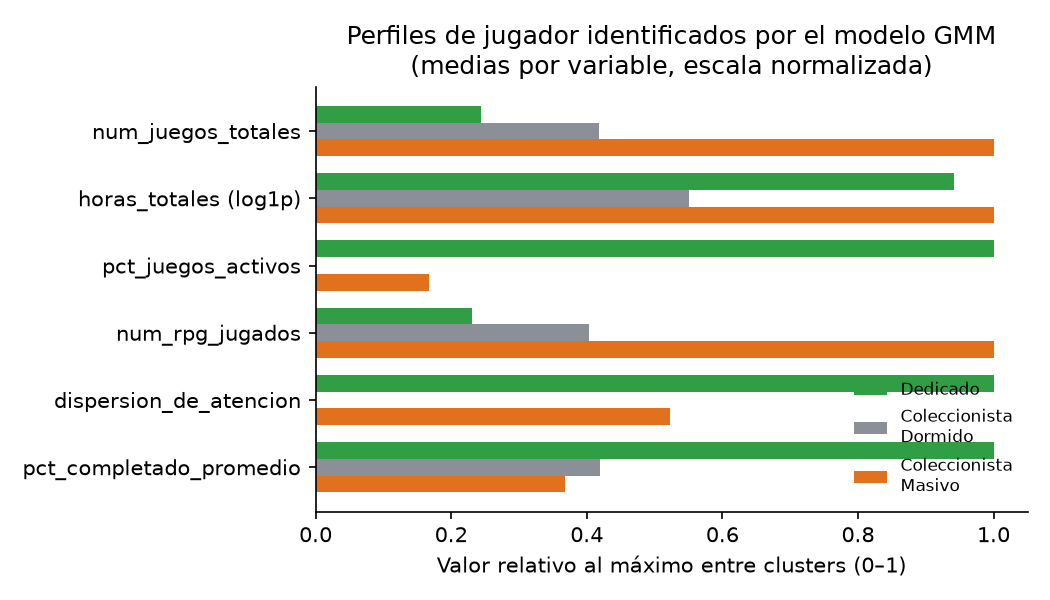
\includegraphics[width=0.85\linewidth]{fig_cluster_perfiles.png}
  \caption{Comparación normalizada de los tres perfiles de jugador según sus variables de comportamiento medias.}
  \label{fig:clusters}
\end{figure}

\begin{itemize}
  \item \textbf{Jugador Dedicado:} biblioteca relativamente pequeña, pero con la mayor actividad reciente y el mayor avance promedio en la historia de sus RPGs (más de 5 veces la duración de la historia principal en promedio, es decir, explora también contenido secundario y rejuega). Es el perfil de menor riesgo de abandono y el más receptivo a recomendaciones de nuevos títulos similares a los que ya disfruta.
  \item \textbf{Coleccionista Dormido:} biblioteca de tamaño medio, pero con actividad reciente prácticamente nula (0\% de juegos activos). Representa al jugador que compra por impulso o en ofertas, pero no consume lo comprado; es el segmento de mayor oportunidad para campañas de reactivación.
  \item \textbf{Coleccionista Masivo:} la biblioteca más grande por amplio margen (más del doble que el Coleccionista Dormido), con muchas horas acumuladas en términos absolutos pero el menor avance promedio por título individual, señal de que su consumo está muy disperso entre cientos de juegos en lugar de concentrado. Es el perfil más sensible a recomendaciones muy personalizadas, dado el tamaño de su catálogo poseído.
\end{itemize}

% ===================================================================
\section{Resolución del problema}
% ===================================================================

Los tres modelos descritos se integran en una aplicación interactiva construida con \textbf{Streamlit} (Streamlit Inc., s.f.), que resuelve el problema planteado en la Sección~2 de forma end-to-end: a partir del identificador de Steam (o URL de perfil) de una persona, la aplicación consulta en tiempo real su biblioteca mediante la Steam Web API, reconstruye exactamente las mismas variables usadas en el entrenamiento (\code{feature\_engineering.py}), y aplica los tres modelos guardados (\code{model\_utils.py}) para producir:

\begin{enumerate}
  \item \textbf{Recomendaciones para comprar} (Modelo 1): un catálogo paginado de RPGs no poseídos, ordenado por menor probabilidad de abandono, mostrando una insignia de ``compatibilidad'' ($1 - P(\text{abandono})$) con codificación semafórica (verde/amarillo/rojo en los umbrales de 34\% y 67\% de riesgo).
  \item \textbf{Riesgo en juegos ya poseídos} (Modelo 2): para cada RPG en la biblioteca del jugador, una barra de progreso de horas jugadas frente a la duración de la historia principal, junto con su probabilidad de abandono, para priorizar qué títulos podrían necesitar un empujón de reenganche.
  \item \textbf{Perfil de estilo de juego} (GMM): el perfil dominante del jugador (Dedicado, Coleccionista Dormido o Coleccionista Masivo) junto con las probabilidades de afinidad a cada uno de los tres perfiles.
  \item \textbf{Asistente conversacional}: un chatbot (modelo \code{gpt-4o-mini} vía API de OpenAI; OpenAI, 2024) que recibe como contexto, en cada turno, los datos ya calculados del jugador (estadísticas de biblioteca, top-5 recomendaciones de compra, top-5 juegos poseídos en riesgo y perfil de cluster), con la instrucción explícita de no inventar datos numéricos fuera de ese contexto, de forma que las respuestas del asistente estén siempre ancladas en predicciones reales de los modelos y no en alucinaciones del modelo de lenguaje.
\end{enumerate}

Esta integración resuelve el problema de negocio de dos formas complementarias: reduce la fricción de descubrimiento de catálogo para el jugador (traduciendo miles de opciones en un puñado de recomendaciones de bajo riesgo, explicadas en lenguaje natural por el asistente), y convierte señales de comportamiento dispersas (horas jugadas, actividad reciente, tamaño de biblioteca) en tres indicadores accionables ---riesgo de precompra, riesgo de postcompra y perfil de jugador--- que pueden alimentar directamente decisiones de retención, tanto a nivel individual (dentro de la propia aplicación) como, potencialmente, a nivel agregado para un estudio o publisher (Sección~\ref{sec:estrategia}).

% ===================================================================
\section{Estrategia}
\label{sec:estrategia}
% ===================================================================

La estrategia de SteamSense Pro está orientada a la \textbf{fidelización de los jugadores de RPG}, entendida en un doble sentido: fidelizar al jugador con el propio género y con su biblioteca (para que efectivamente disfrute y complete lo que compra), y fidelizar al jugador con la marca/estudio detrás del juego (para sostener su relación comercial a largo plazo). Por su naturaleza, la estrategia tiene valor simultáneo para dos tipos de usuario con necesidades distintas pero complementarias.

\subsection{Descripción de usuarios}

\begin{itemize}
  \item \textbf{Jugadores individuales:} personas con una biblioteca de Steam ya establecida (en promedio, decenas o cientos de juegos, según el perfil de cluster) que enfrentan sobrecarga de elección al decidir su próxima compra de RPG, y que con frecuencia acumulan títulos sin terminar. Su necesidad principal es \emph{reducir el riesgo de arrepentimiento} en la compra (``¿voy a terminar este juego o va a sumarse a mi pila de pendientes?'') y \emph{recibir un empujón concreto} para retomar juegos que ya poseen y que valen la pena completar.
  \item \textbf{Estudios y publishers de videojuegos (empresas):} equipos de producto, marketing o \textit{live operations} de estudios pequeños y medianos que no cuentan con un equipo de ciencia de datos propio, pero que necesitan entender por qué su base de jugadores abandona sus títulos, a quién dirigir campañas de reenganche (por ejemplo, notificaciones de nuevo contenido o descuentos en DLC) y qué tipo de contenido futuro (secuelas, expansiones, duración recomendada) tiene mayor probabilidad de ser completado por su audiencia real, segmentada por perfil de consumo.
  \item \textbf{La plataforma (Steam u otras tiendas digitales):} de forma secundaria, un motor de este tipo también sirve al interés de la propia plataforma de distribución, cuyo ingreso depende de que los jugadores seleccionen y disfruten productos, no solo de que los compren una vez.
\end{itemize}

\subsection{Accionables}

A partir de las salidas de los tres modelos, se identifican los siguientes accionables concretos, fundamentados directamente en los resultados de la Sección~\ref{sec:modelacion}:

\begin{enumerate}
  \item \textbf{Para jugadores --- recomendación de compra de bajo riesgo:} usar el Modelo 1 (AP = 0.966, \textit{recall} de 0.741 en la clase ``no abandono'') para filtrar el catálogo de RPGs no poseídos y mostrar en primer lugar los títulos con menor probabilidad de abandono dado el perfil de consumo del jugador, en lugar de solo popularidad o calificación general. Esto es directamente accionable porque el modelo entrega una probabilidad por juego que ya está integrada en la aplicación como insignia de ``compatibilidad''.
  \item \textbf{Para jugadores --- alertas de reenganche sobre su propia biblioteca:} usar el Modelo 2 (AP = 0.999, \textit{recall} de 0.949 en la clase ``no abandono'') para priorizar, entre los RPGs ya poseídos, cuáles mostrar primero como candidatos a retomar, ordenados por menor riesgo de abandono (es decir, los que el jugador tiene más probabilidad de disfrutar si les da una oportunidad) y complementarlo con los de mayor riesgo como alertas explícitas de ``esto lleva mucho tiempo sin tocarse''.
  \item \textbf{Para empresas --- segmentación de campañas por perfil GMM:} dirigir comunicación diferenciada según el perfil dominante del jugador: al \emph{Coleccionista Dormido} (0\% de actividad reciente en el segmento) con campañas de reactivación de bajo costo (recordatorios, descuentos en contenido corto); al \emph{Jugador Dedicado} con anuncios tempranos de secuelas o DLC, dado su alto avance promedio de historia (5.01) y mayor probabilidad de conversión; y al \emph{Coleccionista Masivo} con recomendaciones muy personalizadas dentro de su propia biblioteca (ya posee 145 RPGs en promedio), en lugar de nuevas compras.
  \item \textbf{Para empresas --- diseño de contenido informado por duración:} usar la relación observada entre \code{main\_story}, \code{main\_extra} y la tasa de abandono para calibrar la duración de la historia principal de futuros lanzamientos o expansiones, evitando extensiones de contenido que excedan sistemáticamente el umbral de finalización real de su audiencia objetivo.
  \item \textbf{Para la aplicación --- ajuste de umbral de decisión:} dado que la precisión de la clase minoritaria del Modelo 1 es moderada (0.378), se recomienda como accionable de corto plazo exponer el umbral de decisión como parámetro ajustable (por ejemplo, un control de ``tolerancia al riesgo'' en la interfaz), en lugar de un corte fijo al 50\%, permitiendo a cada usuario u operador de negocio decidir su propio balance entre precisión y cobertura de recomendaciones.
\end{enumerate}

\subsection{Usabilidad del modelo}

La usabilidad de SteamSense Pro se diseñó alrededor de tres principios:

\begin{itemize}
  \item \textbf{Cero fricción de entrada:} el único dato que el jugador debe aportar es su identificador o URL de perfil de Steam (siempre que su perfil sea público); no se requiere completar cuestionarios ni calificar juegos manualmente, ya que todas las variables se derivan automáticamente de su historial existente en Steam mediante \code{steam\_client.py} y \code{feature\_engineering.py}.
  \item \textbf{Traducción de probabilidades a lenguaje accionable:} las salidas crudas de los modelos (probabilidades entre 0 y 1) nunca se muestran como tales al usuario final; se transforman en insignias semafóricas de compatibilidad/riesgo y en barras de progreso de avance de historia, y además se explican en lenguaje natural a través del asistente conversacional, que tiene acceso al mismo contexto numérico que alimenta la interfaz, evitando que el usuario deba interpretar una cifra estadística por sí mismo.
  \item \textbf{Doble nivel de uso (individual y agregado):} aunque la interfaz actual está diseñada para el uso individual de un jugador, la misma arquitectura de modelos (probabilidad de abandono por título y perfil de cluster por jugador) es directamente reutilizable a nivel agregado por una empresa ---por ejemplo, aplicando los modelos sobre una base de miles de jugadores para generar reportes de riesgo de abandono por título o distribución de perfiles de audiencia---, sin requerir reentrenamiento, lo que hace de la usabilidad del modelo una propiedad que se extiende naturalmente de un caso de uso B2C a uno B2B.
\end{itemize}

En conjunto, esta estrategia conecta directamente el desempeño técnico documentado en la Sección~\ref{sec:modelacion} ---modelos con Average Precision de 0.966 y 0.999, y una segmentación de jugadores validada estadísticamente aunque ajustada por criterio de negocio a $k=3$--- con decisiones de producto y de negocio concretas, tanto para el jugador final como para las empresas del ecosistema de videojuegos RPG.

% ===================================================================
\section{Conclusiones}
\label{sec:conclusiones}
% ===================================================================

SteamSense Pro demuestra que es posible predecir con buen desempeño el abandono de videojuegos RPG usando exclusivamente señales de comportamiento públicamente disponibles en Steam, sin necesidad de encuestas ni datos declarados por el propio jugador. Los hallazgos principales son:

\begin{enumerate}
  \item El abandono de RPGs es la norma, no la excepción, en el comportamiento observado de los jugadores de Steam: menos del 1\% de los registros jugador--juego de la biblioteca completa muestran actividad en las últimas dos semanas, lo que valida la relevancia del problema de negocio planteado.
  \item Los modelos basados en árboles de gradiente boosting, en particular \textbf{LightGBM}, superan de forma consistente a modelos lineales (Regresión Logística, LDA) y a KNN en ambos problemas de clasificación, con un Average Precision de \textbf{0.966} en el escenario de precompra y \textbf{0.999} en el de postcompra, este último favorecido por un desbalance de clases aún mayor y por variables de corte temporal más informativas (\code{horas\_hasta\_corte}).
  \item El modelo de \textit{clustering} GMM identifica tres perfiles de jugador con diferencias claras y accionables en tamaño de biblioteca, actividad reciente y avance de historia, aun cuando la configuración desplegada ($k=3$) no es la de mejor puntaje estadístico marginal ($k=2$); esto ilustra que la mejor decisión de modelado no siempre coincide con el óptimo puramente estadístico cuando existe un objetivo de interpretabilidad de negocio explícito.
  \item La combinación de los tres modelos en una única aplicación permite una estrategia de fidelización con valor dual: ayuda al jugador a elegir mejor y a retomar lo que ya compró, y ofrece a estudios y publishers una capa de inteligencia de retención basada en datos de comportamiento real, replicable a escala sin depender de un equipo de ciencia de datos propio.
\end{enumerate}

Como líneas de trabajo futuro se identifican: (i) mejorar la precisión de la clase minoritaria del Modelo 1 (actualmente 0.378) mediante técnicas adicionales de balanceo o umbrales de decisión ajustables; (ii) extender la variable \code{promedio\_pct\_completado\_historia\_global} con el mismo ajuste \textit{leave-one-out} aplicado al resto de variables agregadas, actualmente pendiente por decisión de diseño; y (iii) validar los tres perfiles de jugador con datos de seguimiento longitudinal (por ejemplo, si un \emph{Coleccionista Dormido} reactivado efectivamente reduce su probabilidad de abandono tras una campaña dirigida), cerrando el ciclo entre predicción y estrategia con evidencia causal.

% ===================================================================
\section{Referencias y citas bibliográficas}
% ===================================================================

\begin{list}{}{\setlength{\leftmargin}{1.5em}\setlength{\itemindent}{-1.5em}\setlength{\itemsep}{0.7em}\setlength{\parsep}{0pt}}

\item Chen, T., \& Guestrin, C. (2016). XGBoost: A scalable tree boosting system. En \textit{Proceedings of the 22nd ACM SIGKDD International Conference on Knowledge Discovery and Data Mining} (pp. 785--794). Association for Computing Machinery. \url{https://doi.org/10.1145/2939672.2939785}

\item HowLongToBeat. (s.f.). \textit{HowLongToBeat} [Base de datos de duración de videojuegos]. Recuperado en 2026, de \url{https://howlongtobeat.com}

\item Jolliffe, I. T., \& Cadima, J. (2016). Principal component analysis: A review and recent developments. \textit{Philosophical Transactions of the Royal Society A}, \textit{374}(2065), Article 20150202. \url{https://doi.org/10.1098/rsta.2015.0202}

\item Ke, G., Meng, Q., Finley, T., Wang, T., Chen, W., Ma, W., Ye, Q., \& Liu, T.-Y. (2017). LightGBM: A highly efficient gradient boosting decision tree. En \textit{Advances in Neural Information Processing Systems} (Vol. 30, pp. 3146--3154). Curran Associates, Inc.

\item OpenAI. (2024). \textit{GPT-4o mini: Advancing cost-efficient intelligence} [Comunicado técnico]. \url{https://openai.com/index/gpt-4o-mini-advancing-cost-efficient-intelligence/}

\item Pedregosa, F., Varoquaux, G., Gramfort, A., Michel, V., Thirion, B., Grisel, O., Blondel, M., Prettenhofer, P., Weiss, R., Dubourg, V., Vanderplas, J., Passos, A., Cournapeau, D., Brucher, M., Perrot, M., \& Duchesnay, E. (2011). Scikit-learn: Machine learning in Python. \textit{Journal of Machine Learning Research}, \textit{12}, 2825--2830.

\item Reynolds, D. A. (2009). Gaussian mixture models. En S. Z. Li \& A. Jain (Eds.), \textit{Encyclopedia of Biometrics} (pp. 659--663). Springer. \url{https://doi.org/10.1007/978-0-387-73003-5_196}

\item Streamlit Inc. (s.f.). \textit{Streamlit documentation}. Recuperado en 2026, de \url{https://docs.streamlit.io}

\item SteamSpy. (s.f.). \textit{SteamSpy API} [Conjunto de datos y API]. Recuperado en 2026, de \url{https://steamspy.com/api.php}

\item Valve Corporation. (s.f.). \textit{Steam Web API documentation}. Steamworks Documentation. Recuperado en 2026, de \url{https://developer.valvesoftware.com/wiki/Steam_Web_API}

\item Yeo, I.-K., \& Johnson, R. A. (2000). A new family of power transformations to improve normality or symmetry. \textit{Biometrika}, \textit{87}(4), 954--959. \url{https://doi.org/10.1093/biomet/87.4.954}

\end{list}

\end{document}
